\documentclass[letterpaper,11pt]{article}
\usepackage{natbib}
\usepackage{subcaption}
\usepackage{caption}
\bibliographystyle{unsrtnat}
\usepackage{tabularx} % extra features for tabular environment
\usepackage{amsmath}  % improve math presentation
\usepackage{graphicx} % takes care of graphic including machinery
\usepackage[margin=1in,letterpaper]{geometry} % decreases margins
%\usepackage{cite} % takes care of citations
\usepackage[final]{hyperref} % adds hyper links inside the generated pdf file
\hypersetup{
	colorlinks=true,       % false: boxed links; true: colored links
	linkcolor=blue,        % color of internal links
	citecolor=blue,        % color of links to bibliography
	filecolor=magenta,     % color of file links
	urlcolor=blue         
}
\usepackage{amsfonts}
\usepackage{booktabs}
\usepackage{siunitx}
\usepackage{multirow}
%+++++++++++++++++++++++++++++++++++++++
\begin{document}

\title{HPC-AI Mines Paristech \\\textbf{Machine Learning Project}}
\author{MILLAN Aymeric, VITAL Eduardo, Team AE Dragons\\[1cm]{\small Professor: Nelle Varoquaux}}
\date{February 27, 2022}
\maketitle

\section{Introduction}

The Machine Learning Project consists of a prediction challenge, hosted by the CodaLab platform, for inferring protein functions; more specifically, whether a protein of a particular organism has a particular function. During the project, various machine learning techniques were tested, from data processing to training algorithms, using the \textit{Python} programming language and favouring the \textit{scikit-learn} library. 

The goal of this data challenge itself is to resolve a use case in data analysis which is inspired from a real scientific project (and real data in a simplified form), where the features were extracted from protein sequences of about 300 organisms. Data observation and solution were made available through \textit{protein\_train} files, in which the model should be trained. After that, the model could predict by means of a \textit{protein\_test} and \textit{protein\_valid} data sets and be evaluated internally (facilitated by a submission script), in order to output a final score. This final score is sent to a ranking, defining, thus, the competition challenge.

Our code can be found in
\href{https://github.com/Aympab/ML-project}{this repository GitHub},
you will find more informations on how we processed to get our final models in
the next sections.

\section{Data Analysis and Visualisation}
The first step of the project is to comprehend the data. The training set contains 53118 observations and 952 features, while the output is binary. We can use PCA to reduce the dimensionality of the data in order to do a 3d scatter plot of its 3 most important principal components coloured by its label [figure \ref{fig:3DPCA}]. From this graphic, we can promptly see that each label is not linearly separable from each other, inferring that linear models, such as logistic regression or SVM with a linear kernel, will not do a good classification job. The same conclusion can be achieved through the figure \ref{fig:5DPCA} showing the 5 principal components correlations and the scaling effect on the distribution.


\section{Pipeline}

After understanding our data, we can begin to work on it. As our training base is the only one we have with a corresponding solution, in this first moment it is the only way to also test the performance of the algorithms. However, by submitting a model, we will also receive a score from the test and validation set using the \textit{balanced accuracy score} metric (metric used during all the project).

If we didn't have those extra datasets, we would have to further devise our training observations into another subset in order to test the performance of the algorithm. We chose, nevertheless, not to do this with the intent to optimize our use of data; computing, thus, the score only in the submitting stage.

In order to properly choose a model, a series of operations have to be applied, including:
\begin{itemize}
    \item Pre-process the data.
    \item Grid-search different estimators to optimize its hyper-parameters.
    \item Submit the best model from each Grid-search.
    \item Analyse the best score obtained from the different models, already ranked in the platform.
\end{itemize}

The first two steps can be joined together in a \textit{scikit-learn} pipeline as a means to fit and predict the series of algorithms in only one step.

\subsection{Pre-processing}
As observed, the data has a higher number of features, so it would be a good idea to implement a dimensionality reduction to have lesser features and avoid outfitting. Moreover, scaling techniques are of the most importance to assure that features have the same length.

Therefore, due to the above points and profiting from the fact that some dimension reduction methods require scaling first, we can build a small pre-processing pipeline consisting of scaling and feature reduction.

There are, however, plenty of possibilities for these pipelines using different algorithms for each step. In addition, each one of those pre-processing algorithms can have multiple parameters (hyper-parameters). Our approach to choose, thus, the final pre-processing pipeline, was to grid-search through all these pipelines, but at the end, instead of optimising the hyper-parameters of various predicting estimators, we used only one simple model.

This approach is much less costly and can achieve good results in the choice of the pre-processor. The simple model chosen was a KNN with specific parameters that presented a good performance in previous tests. Other options discussed were decision tree and logistic regression.

For the pre-processing algorithms, the options tested were: Standard Scaler, Robust Scaler, Quartile Transformer, Kernel PCA, Feature Agglomeration and Gaussian Random Projection, resulting in 9 pipelines. Those operations were run locally due to an issue in the CEMEF cluster we are presenting in the next section.

The best results obtained, used in the main pipeline was a robust scaler with feature agglomeration (\ref{fig:PipelinePerf} illustrates the performances), clustering 650 features.


\subsection{Optimisation of Hyper-parameters}

To optimize the hyper-parameters of the different models, we used a grid-search, or even random grid-search, approach. This method was applied for the pre-processing pipeline and also to the training of each estimator. This process was used specifying k-fold cross-validation training, using k=4 usually.

One important point during the utilisation of the grid-search function is to use the pipeline object: fitting the scaling, the dimensionality reduction and the machine learning algorithm at each train set of the cross-validation and applying it to the corresponding test subset. Otherwise, without the use of a pipeline, the fitting of the pre-processing would be done in the whole data set, causing over-fitting in the test subsets of the cross-validations contained in the grid-search.

Nevertheless, this faulted approach was used to enable the use of the CEMEF cluster, where more expensive calculations could be run. This had to happen because, due to memory and C++ libraries issues, a grid-search using a pipeline crashed when run on the cluster.

This grid-searches were trained with different algorithms: Boosted trees (from xgboost), random forest, bagging trees, decision trees, KNN, SVC, neural networks and logistic regression.

Each one of the best models is then trained in the new validation and test data sets for submission. One important point, is that the pre-processing applied in these observations was fitted only in the training ones.

The best of the models submitted can be viewed in CodaLab ranking. Over the best models found, another fine tuning was yet applied in the random grid-search realized in the training set, with a Poisson distribution centered in the best parameters of the estimators. Then, those new models were submitted, achieving a higher score.


\section{Results and Analysis}

The best overall models were the Neural Network (Multi-Layers Perceptron Classifier) and the KNN classifiers. They were combined with the pre-processing pipeline using a robust scaler and feature agglomeration to reduce the dimension of the data. In this way, a final score of around 0.93 could be obtained.

The dimensionality reduction algorithm varied a lot concerning the number of features chosen, probably because of the limited search space constrained by the computational coast. The PCA with poly kernel, for example, took a very long time to fit and transform, so the search space had to be very limited.

Moreover, we can analyse our models with a leaning curve [figure \ref{fig:LearningCurve} and \ref{fig:LearningCurve}]. As we can see, for one of our MLP and KNN models, we have an expected convergence between our training and cross-validations scores. The gap in the first one suggests a small overfit, while in the second case this is less visible. Analysing the curve tendency, however, shows us that, for both models, performance could be improved if more data were to be acquired.

Our final models with the best parameters can be found in the \textit{main.py}
file. Files in the \textit{models} folder are the ones we ran on the CEMEF's
cluster. Finally, you can find in figure \ref{fig:PerfTable} the performance of
other models we have tried. These are the scores before fine tuning the
hyper parameters and were used to compare the effect of scaling and dimension
reduction before fitting. The number after the name of the transformer used for
the reduction corresponds to the main hyper-parameter used
(e.g. \textit{n\_clusters} for FeatureAgglomeration). These scores are based on
local cross validations, thus not involving the codalab score. When no score is
displayed, it means that the estimator did not converge in a reasonable time.

\section{Conclusion}
In the beginning of the project, our approach consisted in trying different models in order to find the best one. Our strategy evolved when we began to simplify some algorithms in order to better understand the data and quicker run tests on it, always prioritizing the use of the CEMEF cluster nevertheless.

In this way we were able to find a good pre-processing pipeline, resulting in better models than previously tested. Those estimators were improved by grid-searches and fine tuned after, always making the effort not to fit any algorithm in the test datasets, for the purpose of achieving the highest score.

\clearpage
\appendix
\section{Figures}

\begin{figure}[htb]
    \centering
    \begin{subfigure}[b]{0.4\textwidth}
        \centering
        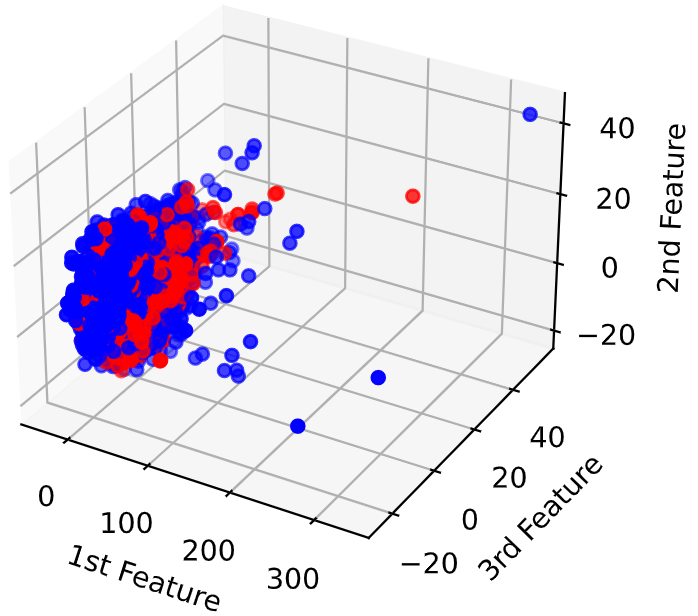
\includegraphics[width=\textwidth]{Images/3DvisuOf3MainFeatures.png}
        \caption{3 components PCA representation: blue=0, red=1.}
        \label{fig:3DPCA}
    \end{subfigure}
    \hfill
    \begin{subfigure}[b]{0.62\textwidth}
        \centering
        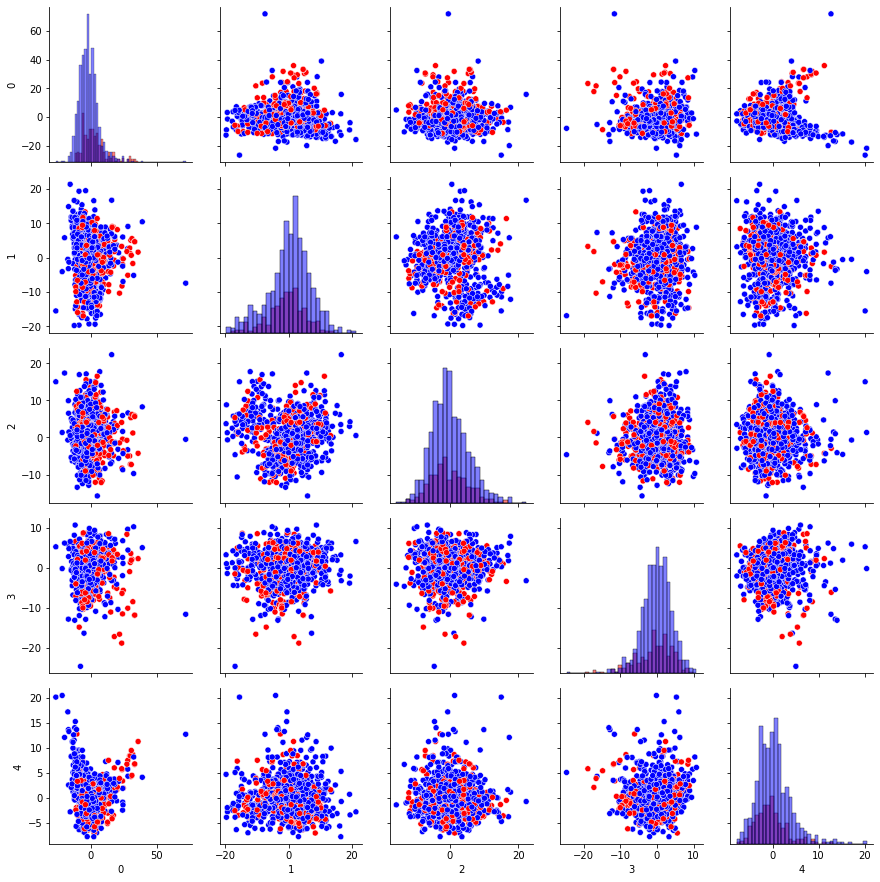
\includegraphics[width=\textwidth]{Images/plot5maincomponents.png}
        \caption{5 components PCA compared 2x2}
        \label{fig:5DPCA}
    \end{subfigure}
\end{figure}

\begin{figure}[htb]
    \centering
    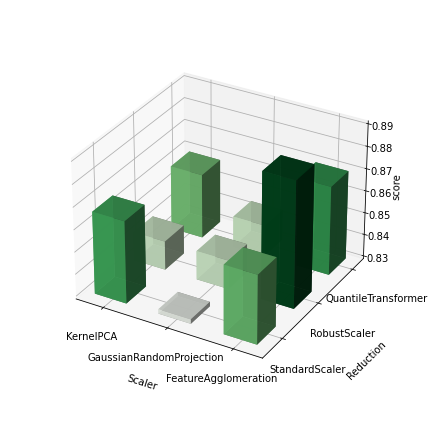
\includegraphics[width=0.6\textwidth]{Images/barGraph.png}
    \caption{Pipeline Scores}
    \label{fig:PipelinePerf}
\end{figure}

\begin{figure}[htb]
    \centering
    \begin{subfigure}[b]{0.45\textwidth}
        \centering
        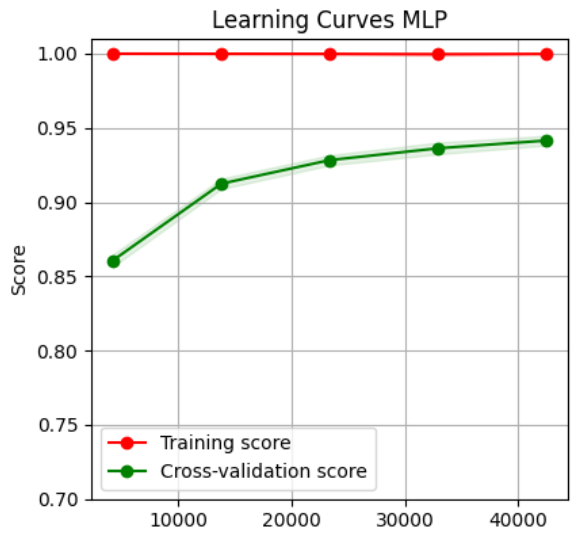
\includegraphics[width=\textwidth]{Images/LearningCurve.png}
        \caption{Learning curve MLP}
        \label{fig:LearningCurve}
    \end{subfigure}
    \hfill
    \begin{subfigure}[b]{0.45\textwidth}
        \centering
        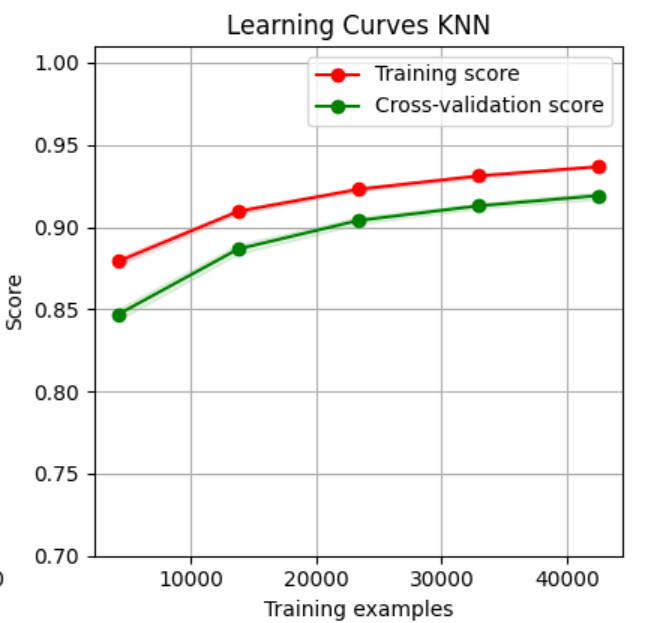
\includegraphics[width=\textwidth]{Images/LearningCurveKNN.PNG}
        \caption{Learning curve KNN}
        \label{fig:LearningCurveKNN}
    \end{subfigure}
\end{figure}

% \begin{figure}[htb]
%     \centering
%     \caption{Models performance table}
%     \label{fig:PerfTable}
%     \begin{tabular}{SSSSSSSS} \toprule
%         {$m$} & {$\Re\{\underline{\mathfrak{X}}(m)\}$} & {$-\Im\{\underline{\mathfrak{X}}(m)\}$} & {$\mathfrak{X}(m)$} & {$\frac{\mathfrak{X}(m)}{23}$} & {$A_m$} & {$\varphi(m)\ /\ ^{\circ}$} & {$\varphi_m\ /\ ^{\circ}$} \\ \midrule
%         1  & 16.128 & +8.872 & 16.128 & 1.402 & 1.373 & -146.6 & -137.6 \\
%         2  & 3.442  & -2.509 & 3.442  & 0.299 & 0.343 & 133.2  & 152.4  \\
%         3  & 1.826  & -0.363 & 1.826  & 0.159 & 0.119 & 168.5  & -161.1 \\
%         4  & 0.993  & -0.429 & 0.993  & 0.086 & 0.08  & 25.6   & 90     \\ \midrule
%         5  & 1.29   & +0.099 & 1.29   & 0.112 & 0.097 & -175.6 & -114.7 \\
%         6  & 0.483  & -0.183 & 0.483  & 0.042 & 0.063 & 22.3   & 122.5  \\
%         7  & 0.766  & -0.475 & 0.766  & 0.067 & 0.039 & 141.6  & -122   \\
%         8  & 0.624  & +0.365 & 0.624  & 0.054 & 0.04  & -35.7  & 90     \\ \midrule
%         9  & 0.641  & -0.466 & 0.641  & 0.056 & 0.045 & 133.3  & -106.3 \\
%         10 & 0.45   & +0.421 & 0.45   & 0.039 & 0.034 & -69.4  & 110.9  \\
%         11 & 0.598  & -0.597 & 0.598  & 0.052 & 0.025 & 92.3   & -109.3 \\ \bottomrule
%     \end{tabular}
% \end{figure}

\begin{figure}[htb]
    \centering
    \caption{Models Performance Table}
    \label{fig:PerfTable}
    \begin{tabular}{@{}|l|lcccc|@{}}
        \toprule
        \multicolumn{1}{|c|}{\multirow{2}{*}{\textbf{Scaler}}} & \multicolumn{1}{c|}{\multirow{2}{*}{\textbf{Reductor}}} & \multicolumn{4}{c|}{\textbf{Model}} \\ \cmidrule(l){3-6} 
        \multicolumn{1}{|c|}{}            & \multicolumn{1}{c|}{} & MLP   & KNN   & XGBOOST & SelfTrainMLP \\ \midrule
        \multirow{2}{*}{QuantTrans}       & FeaturAgg (650)       & 0.893 & 0.892 & 0.871   & 0.88         \\
                                          & GaussProj (700)       & 0.892 & 0.858 & X       & 0.891        \\ \midrule
        \multirow{3}{*}{RobustScaler}   & GaussProj (800)       & 0.896 & 0.873 & X       & 0.900        \\
                                          & PolyPCA (423)         & 0.778 & 0.89  & X       & 0.784        \\
                                          & LinPCA (177)          & 0.887 & 0.879 & 0.844   & 0.885        \\ \midrule
        \multirow{3}{*}{StandardScaler} & FeaturAgg (100)       & 0.878 & 0.893 & 0.868   & 0.879        \\
                                          & GaussProj (700)       & 0.896 & 0.85  & X       & 0.895        \\
                                          & PolyPCA (423)         & 0.772 & 0.898 & 0.873   & 0.773        \\ \bottomrule
        \end{tabular}
    
\end{figure}

\end{document}
